\documentclass[]{article}
\usepackage{tikz}
\usetikzlibrary{shadings, shadows, shapes, arrows, calc, positioning, shapes.geometric}
\usepackage{pgfplots}
\pgfplotsset{compat=1.16}
\usepackage{mathtools,amssymb}
\usepackage[skip=10pt plus1pt, indent=20pt]{parskip}
\usepackage{setspace}
%\input{Preamble}
%\input{(SpecialDistanceCourse}
%\input{FRAMES}
\title{Talk Main}
 \onehalfspacing
 
\begin{document}
\maketitle

\section{Introduction} 
We know we are in a housing crisis, housing is becoming increasingly expensive relative to income, and more people lack access to adequate housing. In this thesis, we are looking at the urban and economic dynamics that are driving the crisis and how these dynamics are going to affect the larger system.

One major driver of the crisis is the financialization of housing. Financialization is the capture of flows of surplus by financial actors. CUT. %And it’s achieved through the creation of financial instruments that allow the capture of that surplus value. 
I wanted to look at the financialization of housing, 

I set out to assemble a model that can describe how the financialization of housing affects the city. %This is a theoretical project 
The model had to capture what drives urban productivity and growth. It needed a labour market, a spatial housing market with capital gains and locational rents, and an explicit mechanism for determining housing ownership.

There are two key insights about cities that underlie our approach:

\begin{enumerate}
    \item Cities generate a surplus. One of the most robust empirical regularities in ??? is that the productivity of cities increases with population. The relationship is a power law relationship. %In standard economic terms,
    Economists would say cities show increasing returns to scale. (PLOT)

    \item Cities are both economic engines and spatial entities and that duality is key to housing markets which are fundamentally a spatial kind of market, and space plays a role in who can claim the surplus. So to understand what’s happening in these markets, we need to take into consideration both the production value and how it is organized within space.
\end{enumerate}

The challenge was to bring together the logic of the spatial relationships, well described in urban geography and economics with economic logics of production and finance that are generally modelled as spaceless.

The result is a model with three components:
\begin{enumerate}
    \item how value is created in cities
    \item how spatial urban land rents play a role in distributing that value and
    \item how actors capture the value through housing markets.
\end{enumerate}
The model allows us to explore how financialization affects who owns property, and get at this question of who is capturing the value produced in the city.

For this talk I will:

\begin{enumerate}
    \item Set up the theoretical foundation. CUT Start by going through the key ideas that form the theoretical foundation for the work: financialization, spatial rents, and growth.
    \item Describe how we’ve brought these together in a model CUT elements together in a simulation model
    \item And discuss the results that we get from the model. CUT?? Theoretical foundations I think this is done above
\end{enumerate}

\section{ THEORY}
For the theoretical foundations we need three concepts from three distinct literatures:

\begin{itemize}
    \item financialization
    \item spatial rents and
    \item growth
\end{itemize}

The relationship between productivity and financialization may not go in just one direction, so as part of the theoretical foundation, we consider the possibility that there is a linkage where financialization may affect productivity.

\subsection{Financialization}
Financialization is the capture of flows of surplus by financial actors. 
It’s achieved through the creation of financial instruments, like REITs, and mortgages, that allow the capture of that surplus value.

In the case of the city, the surplus that financialization is capturing is the productivity that we understand as coming from bringing people together in the city. We argue that one mechanism of claiming surplus works through land rents and is at the heart of what’s happening in urban centers. 

We haven’t found formal models that introduce financialization into an urban production economy. We have seen work that examines the data and proposes a similar explanation- for example, Jeremy Withers a housing policy researcher and PhD Candidate at the University of Toronto. 
Putting these pieces into one model as I do makes it possible to explore how the pattern plays out over time, and to explore the effect of policy interventions.

\subsection{Spatial rents}
In order to model the capture of surplus through land markets, we need to understand how value is distributed through space. We have two sources - classical economics and modern urban geography.

The first is \textbf{from classical economics}: we borrow Ricardo's theory of land rent. David Ricardo provided the canonical theory of rent in his Essay on the Influence of a Low Price of Corn on the Profits of Stock in 1815.

We can illustrate Ricardo’s theory with the story of a carter who purchases produce at the farm gate and has a cost to transport them to the market. The farther he has to travel, the less he will pay for produce at the farm gate. The lower the price of the produce, the lower the value of the farm. Land value thus depends on the distance to the market.

Ricardo’s theory of rent generates a theory of distribution, with all the surplus going to landowners in the form of rents. 

Ricardo was describing what was still basically the feudal part of the economy. Later in the 19th century, with industrialization, economic theory shifted to focusing on production with produced capital instead of natural capital.

In \textbf{the neoclassical theory of distribution} that developed,(eg John Bates Clark (1847-1938)), space and land no longer played the central role in production or distribution. Workers got the marginal value of their contribution to output and the surplus went to the owners of capital in the form of profit.  (Removing the land removed the role of space.)

In the early 1960’s space and transportation became a focus for urban theorists. Alonso and others modelled urban land values based on the distance from the workplace. This is basically Ricardo’s model relabeled and the urban locational rents rents are simply Ricardian land rents.

In Alonso et al model, jobs are at the center and people have to pay to get the work. There’s a maximum distance that it’s worth travelling to work. That determines city size. It also determines land prices since workers will pay to be close to work. By the 1970s this was the dominant model in urban economics. 

The model did not explain urban productivity nor did it grapple with distributional issues as Ricardo had. 

\begin{table}[h!b]
    \centering
    \begin{tabular}{r|ccc}
         &\multicolumn{3}{c}{ MODEL} \\\cline{2-4}
Feature   &Ricardian   &Neoclassical &Cities \\\hline
inputs    & land, labour & capital, labour&land, labour, capital\\
incomes   & rent, wages  & profit wages &rent, wages, profit \\
space is  & essential   & suppressed& essential\\
    \end{tabular}
    \caption{Ricardian, Neoclassical, and urban production and distribution}
    \label{tab:my_label}
\end{table}

\textbf{Our contribution} is to combine the Alonso-style theory of urban land rent with neoclassical production and a Ricardian treatment of distribution.
We recover the channel of distribution running through land. 
That channel is largely ignored in both neoclassical models and in modern urban theory.

\subsection{Growth}
We still need to build in the economic dynamism of the city. 
How do cities produce value? 

Growth theorists observed growing productivity over time \textbf{at the national level}. This was a puzzle given they were modelling an economy with decreasing returns

Jane Jacobs observed that increasing returns applied \textbf{at the city level} and  recent work on urban scaling (originating with the Santa-Fe institute) has gone a long way to confirm her view.


Economists have thought about these scaling effects for more than two centuries. Smith talked about specialization giving rise to gains from scale. Marshall noticed that firms and in industrial districts tend to concentrate and scale up, that is they showed increasing returns at the level of the industrial district. More recently explanations have shifted to human and social capital.

The reason for these scale effects may be technology, networks, growth of human capital, or the combinatoric expansion of possibilities as people come together. 
Whatever the cause, these system-level or macro effects are now generally ascribed to ``agglomeration effects''  that are not in the classical or neoclassical model.  

%It has to do with the fact that increasingly wealth comes out of human creativity  HUMAN CAPITAL

% THE SCARCE factor was land

% Then the scarce factor was essentially produced capital- could produce lots- once you have lots of productive capital producing a. huge factor

% the factor that became most important was the creativity of people

% it’s the long-term factor at each point, whereas produced capital is the short term limiting factor.

% cut. culture as a factor of production - works at the general level.

\section{Formally modelling production and growth with DRS firms and IRS cities}
Here’s the equation that’s been estimated in the scaling literature,. As long as that beta is greater than one, the productivity gets bigger as the population increases.


\hspace{4cm} equation

\noindent This says that bringing people together raises everyone’s productivity. It says there are increasing returns to urban labour. There are no firms in this formulation

Growth theorists addressed this using a formulation for the firm that’s become pretty standard: the Cobb-Douglas production function.

\hspace{4cm} equation

\noindent This has diminishing returns at the firm level. According to the theory the wage is the VMPL, so we a theoretically consistent way to derive the wage

We can show the two equations are nested in the following of the same model.

\hspace{4cm}our equation

\noindent We make the productivity term depend on urban population. If population rises, wages rise.

This is now a linked firm-city model of production with DRS for the firm and IRS for the City

\subsection{RENTS}
With this model we can make the link to urban land rents. There is a simple equation for rent at any distance that comes from Alonso et al

\hspace{2cm}EQUATION:  RENT = wage premium - c d

\noindent The wage premium is the extra pay needed to get enough people to work in the city, and pay transportation cost. cd is the transportation cost. land rent is what is leftover after paying transportation costs to get to work.

That’s how much the land owner could charge for use of the location - Whoever owns the land gets the locational rents. not the total rent paid, this is the Ricardian rent (People can get confused here over rent for a building and the locational rent.)

Locational rents come out of the wage premium, which comes out of the surplus product generated by the agglomeration effect!

\subsection{POPULATION}

To close this model we need to link the population and the wage. At the edge of the city there is no urban rent, so we can calculate d from the equation above. That gives us the area of the city and if we know the density we can get the population and plug it back into equation (3)

%$CUT. What we’re doing with this model is putting an urban model of production together with, a formulation of urban rents, and land market with particular mechanisms by which financial and other actors can gain

\subsection{FINANCIALIZATION}

In my model, rising productivity generates capital gains because the rising wage increases land rent. The prospect of capital gains attracts speculators

If we let financial actors buy the land, they can capture the benefits that come from bringing people together.

It’s important to note, that the process of claiming rents that we model here is orthogonal to the process of investment for growth. Investing in productivity and investing in rent capture are two different ways to use financial assets.

%CUT. Actors may invest not just in speculating rents, but in building new housing, upgrading properties, etc. Some of that value provides amenity, creates the conditions for productivity and thriving, some of it increases the supply of housing, some may displace residents through a gentrification.

One of the contributions of this work is to carefully dis-aggregate the two, which are typically lumped together, so we may consider creating value for the city, and taking value out of the city separately. 
This could make it possible to design interventions that can more effectively encourage the kind of investments that create value.

So that gives the theoregical foundation of the ase model.

\subsection{Financialization and Productivity} 
Rising productivity attracts speculators and the financialization of the housing supply. 
Could this relationship go both ways? Could financialization affect productivity?

If the urban surplus is extracted, people in the city have fewer resources to invest in education, developing human capacity, and sustaining the infrastructure that makes the city productive. In the thesis, I identify a number of other channels through which that feedback might happen.

\hspace{2cm}FLASH THE CHANNELS FIGURE, PAUSE 5 SECONDS.

This leads us to ask “What would happen to all of these results if there is feedback from financialization to productivity?  
This is a new question. 

Given the importance of cities. and urban productivity it is potentially very important to have answers. There seems to be a gap in the available theory, empirical work, and policy analysis, so we conduct a Gedankenexperiment. We add a link to the model and see what it does.
    \begin{quotation}
    Gedankenexperiment, (thought experiment) a hypothetical situation in which a hypothesis, theory, or principle is laid out for the purpose of thinking through its consequences.

    A term used by German-born physicist Albert Einstein to describe his unique approach of using conceptual rather than actual experiments in creating the theory of relativity.
    \end{quotation}



I’ll show the world is very different for policy-makers if the productivity linkage is strong.

\section{The Simulation Model }
So far I have been talking about the general theories the simulation model will be based on. This figure shows the main logic of the simulation:
%I set out to assemble a model that can describe how the financialization of housing affects the city. This it a theoretical project The model has to capture what drives urban productivity and growth. It needs a labour market, a spatial housing market with capital gains and locational rents, and an explicit mechanism for determining housing ownership.

\hspace{4cm}SHOW ODD figure%{fig/ODD}needs package for slides

%\noindent I’ll go through the logic behind the flows in the figure

% the core Alonso Jacob mechanism.

% The relationship between agents in the housing market

% What the housing market is doing,

\noindent \textbf{First, the core Alonso-Jacob cycle}. (mostly equilibrium analysis) This is the piece that links labour back to land

Alonso Urban Model: \textbf{wage→ extent → population} %{\tiny(only pop is ABM agents choose to work in the city)}{}

Jacobs Agglomeration: \textbf{ population → productivity}

Neoclassical Production Function: \textbf{productivity → wage setting}

\hspace{4cm}ALONZO JACOBS FIGURE. %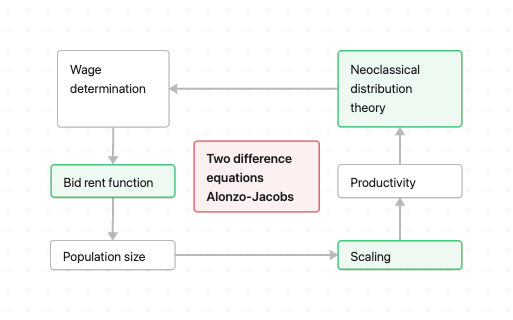
\includegraphics[scale=.2]{fig/flow_Alonzo-Jacobs_cycle.png}

\begin{itemize}
    \item  there is a rural wage. It pays for house, food and living expenses. 
    \item Everything above this is the \textbf{urban wage premium}. The wage premium pays for travel and locational rents. It determines the size of the city.
    
    \item The wage is driven by productivity. 
    
    \item Productivity is determined in part by city population. 
    
    To keep the focus on ownership, the city has

    \item property sizes are all the same

    \item transportation cost is the same for everybody.  All the workers the same.
\end{itemize}

\subsection{ What happens in the housing market}
The second block I’d like to describe is the relationship between the housing market, the bank and buyers. 

\begin{itemize}
    \item People choose whether to work in the city. They can buy land or become tenants
    
    \item Workers have to get mortgages,

    \item Investors can buy land.

    \item investors get loans. Agents decide if a particular property when it comes up is worth purchasing.

    \item Agents calculate the financial value of a purchase including capital gains for each piece of property.

    \item Agents bid in a competitive market.

    \item A bid and auction process allocates each property.

    \item There are parameters to adjust the various costs of capital, how willing banks are to lend to workers, how willing they are to lend to investors, and so on.
\end{itemize}
The market does two things. It allocates the housing between owner occupiers and tenants but it also allocates the locational rents between owner occupiers and investors


\hspace{4cm} HOUSING MARKET FIGURE %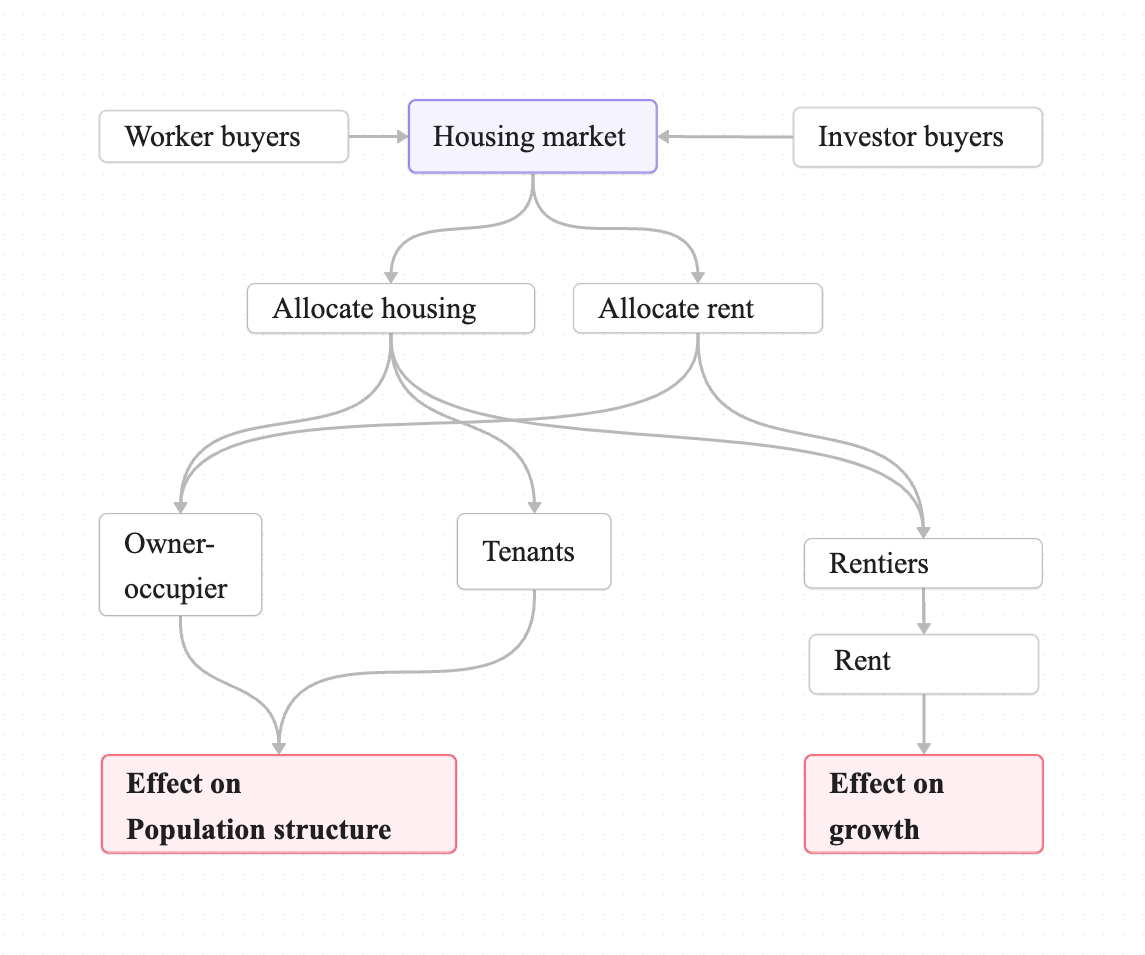
\includegraphics[scale=.20]{fig/flow-impacts.png}?
           
% 1. mention how each decides?

% 2. elaborate as much as you have time for


{\color{orange}: local summary So the structure then on one side is the urban production and agglomeration effects, drawing on Jacobs’ work, growth theory, and the scaling literature - how the city makes value. On the other is the spatial structure of rents drawing on Ricardo, classical rent theory and Alonso’s model of rent in the urban center - how it distributes that value through space.}


%We have a mechanism that is inspired a little game theory and bidding theory to select the winner in these bidding games.


%So that’s our financialization component. Essentially, do the investors have an advantage at some point over the worker buyers? If the investors have an advantage, then they’ll buy an increasing fraction of the housing stock over time as people retire and as new housing comes into the market?

%Finally, let’s just discuss a little bit what the housing market is doing. We’ve got two kinds of buyers as I’ve said.

\hspace{4cm}FIGURE ?

 %CUT. Investors are different social class called rentiers. Now, this is standard economic terminology. rentiers are people who are living off rents than any action they take to create value for others. So that means that they

% Investors are extracting rents from the urban system.

% And that could have an effect on growth. So we have two fundamental outputs of this model, the production story and the distribution/population structure

I start with a city of all owner-occupiers. We want to see if this situation lasts, if we get a mix of owner-occupiers and tenants or if we get all tenants. It makes a difference because these are, in economic terms, different classes with different opportunities. With tenantization  
the wealth created by the city is increasingly transferred from workers to investors. Very simple story. 

%So that’s the basic model.

??? So here’s the flow diagram for how this comes together in the code

% integrated with the equilibrium reasoning the model of the firm. similar approach in that we use relatively standard reasoning, but carefully built from the ground up.
% And again it- urbansim - model of data-Dawn working with him for Toronto. I’ve hosted conversations with 4 or 5 local developers developing proforma for a Waterloo context. can link.

%can build on Dawn, Urbansim, Corsica group, workshop also had collaborators from Doynes group at Oxford join. you may know better the current work at that group. But Dawn and Corsica collaborators, and we are working on one on the SLUCE market that will feed into that. interesting features - linking rental markets etc.
% LAND MARKET MODELLING. also transportation etc.

% In each case, built a carefully grounded .. similar approach in that we use relatively standard reasoning, but carefully built from the ground up. relatively simple, but constrained tightly to the core purpose.

% Fits with the purpose of this model is ‘theoretical exposition’ - extension beyond, keep it simple.

% Three pieces of the model


% sensitivity- study non l inear dynamcis cysters, characterise introduce data.
% And can use them with people. - in lab as boundary objects for communcitaion. to make ideas explicity - LAB GROUP POHOTO
% Firms
% Firms- explicit firm models.. Axtel sat 129 million firms- a platform - very good time to work with that kind of data
% central bank expanding how ti does this kind of modelling.- from representative firm models- - 2-3 countries beginning to explicitly model firms.
% City
% Working with dawn- city - partnership proforma California lang group. met with developers sharing pro-forma. - review of 5 main land models- publishing with Dawns. - Rental markets, development etc.

% Also in practice - some work with the Devco- and HIRT model, and with Maryam - national stratgety for a new normal pattern of development. Ian Bird.

% Institutional linkages

% Much more explicit - SOCIAL INNOVATION IS - change in routine resource flows

% in practice - a fund with a concessionary layer of finance for non-market- get at core– but also actually creating a different class of actors- different flows and relationship.. all the non-market actors in Hamilton conveined so it’s a 500m-2b fund - vs xx billions of federal investment – but not just trying to move through the market- actually using that as part of an implicit model with relationships, actors, routines relationships and paradigm – prioritizing not just the state but the resilience of the state and set of relationships.

%this is part of it because - there are a small set of canonical models- holding in relation with that- integrated with the advantages of precision and long run trajectories– with distributional effects - over people but an extensible- people do things believe things - rules can stop– and the model is shareable like a toy.

\section{Results}
The model's parameter space is large. 
There is a region in this parameter space that gives us the kind of behaviour we expect of a medium-sized growing city. Points in this reproduce the stylized facts about production and city growth. I am going present results from a particular spot in this region of the parameter space. This fictional city is  background for our exploration of the housing and financialization sectors.
%?? It will grow over time and eventually reach a limit size. We aren’t interested in the endpoint - we are interested how financialization and public policies affect its growth path.

Around this point, we explore six policies that are available to the public sector. We’ve chosen these particular policies because they are discussed they’re considered likely to be important.I vary the six parameters that represent policy variables individually.  (These orthogonal explorations are like walking some distance north, south, east and west from a house you are visiting.)

We look to see whether the model behaves plausibly and
whether we get dramatic effects from any of the policies within this plausible model. I will be reporting comparative dynamics results - how the interventions affect the evolution of the city over 100 periods. 

\section{Results}
%\documentclass[]{article}
\usepackage{tikz}
\usetikzlibrary{shadings, shadows, shapes, arrows, calc, positioning, shapes.geometric}
\usepackage{pgfplots}
\pgfplotsset{compat=1.16}
\usepackage{mathtools,amssymb}
%\input{Preamble}
%\input{(SpecialDistanceCourse}
%\input{FRAMES}

\title{Talk Main: Results}
\begin{document} 
\maketitle
\section{Results}%.   comment out lines 1-14 and end{document} to merge
I will only give you the most interesting results. The output tracks seven variables over time for each policy variant. So 6x7x2.5 (2.5 is the average number of policy variants) = 105 plots. Since we look at two versions of the world - one with a productivity linkage and one without - I have over 200 results to summarize. 

}A general observation to start with is that with no linkage, most financial policy changes do not affect the city size, wages . Real-sector policies, like transportation costs and density regulations do affect city size, wages and number of firms

The first new information is that the owner-occupier share drops over time if financialization of the housing market is permitted. 
In the model that we use as a baseline investors eventually capture about 40\% of the housing stock at the end of our run. ??? The speed of the effect is sensitive to the initial point in the parameter space chosen.
This is what are observing happening in the real world, we expected it, but
it emerges endogenously in our model as a result of the way individual behaviours are specified. 

%I think it is important to remember the literature hasn’t actually explored financialization empirically to in great depth, so we don’t have empirical values for the response of many of these variables.

% \section{New Pass 2024-03-16, 3:06 PM Sat}
\subsection{The policy intervention}

\subsubsection{Capital Gains tax on investors}

The very first policy result is that, in the base model a capital gains tax on investors does not affect any of the parameters of city size, number of firms or population or the wage in the community, but it can have a very large effect on the owner-occupier ratio.

If 100\% of capital gains are taxed, there will be no investor participation in the market. And if zero percent are taxed, the rate of investor ownership goes to 100\%. Those are startling results.

This is  interesting at the moment because the federal government has announced it is extending  the capital gain inclusion by 33\%. That  does remove some of the financial incentive for non-productive investment. Our model is too simple to tell us whether it will work or how fast

\subsubsection{Capital Gains tax on owner occupiers}

What would happen if we increase the capital gains for owner-occupiers on on first homes? As the capital tax capital gains rate rises for owner occupiers the share of owner-occupiers falls.

When the capital gains tax gets above the level of the rate paid by investors, the investors take everything. They then have a tax advantage in relative to owners.

%(??? A surprising result is that there is some variation in our model in population.)

\subsubsection{Costly capital for investors}

We need to be clear what the definition here is. It’s just the interest rate that is charged to people, not as homeowners, who borrow to invest in properties (* The rate at which the bank will give them money. They have to beat that rate.). ]

We expect it to affect the home-ownwership rate a little bit.

These results are very minimal. The rate does not appear to make much difference even over a very wide range of rates. We are surprised about that.

It suggests that the capital market access to the capital market is not what determines the attractiveness of investment in housing. We saw that changes in the capital gains tax made a big difference. That leads that tends to support the view that people are investing for capital gains.

(I think these results are a little bit funny,)

\subsubsection{Transportation costs  determine the population} 

If you decrease the transportation cost, the population should go up, and that’s exactly the result.

The only question you might ask is how does it affect the ownership ratio? What we see is that with a reduced cost of transportation, the city grows more, and more of the housing is taken up by investors.

This makes perfect sense. If the city is growing then there are quicker capital gains from investing. To pull in people in the wage has to increase increasing, which means rents can increase.

\subsubsection{Density}

A policy now being pushed quite energetically by the federal and provincial governments.

In our model it is like changing the lot size but assuming each property has the same amenity.

The effect on the housing proportion is not as easy to predict. We can account for it by noting rising capital gains in this model.

If you just increase density, you would expect the city extent to stay the same. That’s what we get.
Changing density does not change the ownership ratio. This is kind of interesting.

The transportation costs rents are not changed at the same location, so the land rent PER UNIT are the same for each person because the transportation cost at that point has the same value. So density does not change the ownership.
The may be twice as many people per unit of land, however, so there Is twice as much locational rent to collect.

That is an interesting result. Once you’ve seen it, it’s not hard to explain.

??? It will be modified by a number of effects, like the cost of converting housing if you’re changing from low density to high density that’s worth exploring further. But the baseline is it does not affect rents.

The effect of asset requirements on home buyers. make this shorter? cut it to save time??

??? (Related to the stress testing of buyers to avoid defaults.)

Banks look at the wealth and incomes of households. In this experiment, we just tighten the savings requirement.

This has almost no effect on the ownership rates.

The most likely explanation for this is that a large supply of people with high enough savings to purchase. We may have a slight shift towards wealthier individuals.

\subsubsection{Property tax rates}

The annual tax paid is a share of the property’s total value. So it can be understood as a deduction from the value of the property and a deduction from the potential capital gains. A. very high property tax rate capturing all the value of the property which is essentially all the capital gains.

10\% is relatively high, (unrealistically high, actually)

The property tax rate has a small effect on population that looks very, very much like what we have in a previous figure for capital tax capital gains tax on owners.

You would expect, in fact that this would work very much the same way as capital gains tax on owners. It looks similar but it has a much bigger effect on the ownership ratio.

What we’re seeing in this case is IF the property tax ratio falls, the ownership ratio falls earlier, but stabilizes on the other hand, if the property tax rate is low, and it drops capital the property tax rate is low.

The ownership ratio begins to drop later but drops farther.  That suggests that the main play here is profitability for investors, which again, reinforces the notion that what’s happening is the capital gains to investors.

So we’ve gone through the list of simple reactions with no feedback. Remember: none of these policies affected the basic economy, but some ded affect the ownership ratio.

\subsection{LINKAGE EXPERIMENTS}

The maintained hypothesis for the following experiments is that, for some reason, an owner-occupier population either invests more or is more productive than a tenant population where the surplus is extracted. 

to get clear effects, we consider a large very simple feedback: if all of the housing is owned by investors, The scale factor $A$  falls by about a third.  Smaller numbers will have a smaller effect, but they will be qualitatively the same. 

Unlike the case with no feedback, as investor ownership rises,  we see

\begin{itemize}
    \item Lower wages.
    \item Lower population,
    \item smaller city
    \item a higher proportion of owner-occupiers
\end{itemize}
The effects don’t kick in until the investors enter the market. When we get to the point where investors start to enter the market and convert housing from owner-occupied to tenant-occupied, productivity declines, the wage basically goes flat, the city stops growing and the population goes flat.

Why is the ownership ratio higher in this case? Shouldn't every indicator be worse?  A smaller city with lower growth generates smaller capital gains. There is less investment so the investors don’t take over as much as the housing as when it keeps growing.
??? Investment is in some sense, self-limiting: once it’s killed off the growth and slowed the city down there’s no longer any reason to keep buying housing.

\subsubsection{Linkage with Capital Gains Tax on Investors}

Keeps all the investors out of the market, so the how the housing stock stays 100\% owner-occupied. We basically get the no linkage effect. A 100\% gain capital gains tax cancels out the effect of the investment link by keeping investors out of the market.

If you lower it to 50\% with the settings we have once investors start to enter the market, you’re your wage goes flat. Your population goes flat, your city extent goes flat. But since they have entered the market, they take up about 40\% of the housing stock.

If the capital gains tax is lower than the capital gains on a principal residence you see a complete takeover the housing stock and the city shrinks sharply once the linkage kicks in.

??? The population grows on the original path at first. It shrinks once the investors come in. Land speculation has an absolutely parasitic and destructive effect on the city

\subsubsection{Linkage with Capital Gains Tax on owner-occupiers}

There is really one result here: When you put a capital gains tax on owner-occupiers  that is higher than the capital gains tax paid by investors, Wage growth flattens out and then drops.

Population drops

Ownership shifts to the investors it becomes a tenant city.

We present results for just two values above the investor rate and two values below it.

So this is interesting because appears that what matters is whether or not investors have a financial advantage over homeowners in the in the market.

CUT. The ownership crash then cuts the productivity that’s the mechanism that this model is exhibiting.

The difference from the no-linkage case that is most notable is that even with a very low capital gains tax on owners, once some of the housing is captured by investors, productivity falls and therefore the wage goes flat.

\subsubsection{Linkage with The cost of capital for investors}

It doesn’t appear that this policy instrument (the cost of capital for investors eg REITs and others wishing to speculate in housing) is very effective. That’s that’s the news.

??? When there is no linkage we could push the cost of capital way up or down, and it had some effect, but it was pretty minimal.

? With the linkage with or without this policy, we get the same levelling off of the wage of population and of city growth. We get less effect on the ownership ratio with a linkage but basically the same pattern as before,

\subsubsection{Linkage with Transportation cost}

With linkage this throws up a new and interesting result.

Reducing transportation cost causes the city to grow in extent as before. Small influences on transportation costs still have a large effect on population.

The new point is that with low transportation costs we get oscillations in the population. (see *** V)

It appears from these runs that the ownership ratio is a little bit higher with a high transportation cost and that’s because of the high transportation costs we have a smaller city and less reason for this thing and it doesn’t grow as fast.

\subsubsection{Linkage with Density Variations}

Pretty much the same result as with no linkage. What is of interest is that the linkage tends to put in more oscillation in these values.

*** It looks like we get a series of speculative booms that cause the city to grow and shrink. Speculation is not causing the growth. Speculation in this model decreases productivity and so you get a decline and then a period with renewed growth that induces more speculation and then a new decline.

\subsubsection{Linkage and the Asset requirement}

No new interesting results except a higher level of home ownership, which I have explained in the other cases: smaller growth, less reason to speculate.

\subsubsection{Linkage and the property tax?}

XXXX. It proved to have some interesting and not easily predicted effects in the no-linkage example. In this example we get similar results:  wage growth flattens with the property tax, and a higher property tax rate reduces the wage to even higher property tax rate.

Why does it reduce the wage? Because it reduces city growth. ???? Smaller city -> lower wages. It reduces the population.

It is interesting that the lowest property tax rate introduces an oscillation as you’ve seen in other examples. This suggests there is a fairly sizable regoin of the policy space - even of the parameter space - that will produce speculation-driven cycles of growth.

A low enough property tax rate does leave you with a higher wage and a higher population
I think I have to go over it again.

\subsubsection{A Transitory Shock}

All the interventions so far have been introduced when the city was born and maintained forever. We can explore short-term policy shocks with this model.

Consider a city that starts with a 100\% capital gains tax at the beginning, removes it for 25 years, and returns to the original 100%

Predictably, when we move the capital gains tax there’s a big influx of investors buying a property. Productivity falls, the wage falls, the population falls. So reducing the capital gains tax dramatically on property has the effect of reducing wages, city size and generally inhibiting growth.

In a similar experiment, with a much longer time horizon to get some sense of what would happen if we reduce the lag rates in the economy if it responded faster, or if we let it run farther.



\end{document}
% remove 

\section{CONCLUSION}

LOVE THIS FOR INTRODUCTION - Cities account for most of the production, housing, and wealth distribution for humanity in our century. They are our dominant economic-demographic form. Growing and changing inexorably they still evade any fully satisfactory description. Despite research over literally centuries and across many fields, they remain somewhat mysterious.

There is a SPECIFIC gap in the formal apparatus in standard economic theory for analyzing the distribution of the enormous value produced through the economic activity of cities.

To at least partly bridge this gap, I have presented a model that combines components from several different fields that grapple with the nature of the city.

From Jacobs, the scale literature, and neoclassical growth theory. I take the agglomeration effect., which I incorporate into an Alonso-style city to explain its growth

From neoclassical production theory, I take the firm production model and wage setting model and add them to the urban model

From Ricardian rent theory. I adapt a model for the distribution of the locational rents generated by urban agglomeration.

On top of this, I build a ABM model of the mortgage and housing markets with two classes of buyers.

The overall goal was to provide a theoretically grounded model of the relationship between financialization and urban productivity and class.
The model highly modular. There are substantial opportunities to extend this work.

% Both the model of the city and the institutional link can be replaced with different models, better data brought in etc. 
% I haven’t YET?? found another model that has production, financialization, and distribution and integrates neoclassical and agent-based modelling te

The model as it stands tells us that financial interests are likely to take over most of the land and capture much of the surplus generated by the city.

These results are based on descriptions of what agents do at the micro level, not on an a priori description of the model dynamics.

At the very highest level of generality this result appears to point to an expansion of rent-seeking financial capitalism that will transform cities and our socio-economic structures. social structure.

I have presented this model in the context of a widely-felt housing crisis to explore how the capture of urban value by financial actors through the financialization of the housing market affects ownership patterns in urban areas, and the probable implications of these processes for urban productivity.

I have designed the model to allow us to explore a variety of policy interventions. One essential result is that policies will have different effects if financialization has an influence on urban productivity.

To end, I would like to call attention to how this project fits in the development of economic theory.

Ricardo produced a spatial theory of production using land and distribution think — of it as a theory pair.
Neoclassical economists produced a spaceless theory pair with production using capital and distribution.
Essentially what the neoclassicals did is drop land, a form of natural capital, out of the production model produced captial

Alonso in effect opened way to reintroduce land and the channel of distribution that runs through land.

My model adds that channel to a neoclassical model with financialization.
??? The land that was removed in the analysis of industrial society has to be put back in to understand urban society. Land is a hidden factor of production in the neoclassical model. It contributes proximity to workers. CUT. It is a complementary factor that can be left out is it is simply proportional to the numbier of workers but It can’t be left out if there is a feedback from land through population to productivity - the Jacobs link.

So let me thank you there and I’ll take questions.



\end{document}